\documentclass[12pt, a4paper]{article}
\usepackage[margin = 1in, top=1.3in]{geometry}
\usepackage[english]{babel}
\usepackage[utf8]{inputenc}
\usepackage{fancyhdr}
\usepackage{amsmath}
\usepackage{bm}
\usepackage{graphicx}
\usepackage{subcaption}
\usepackage[font=small,labelfont=bf]{caption}
 
\pagestyle{fancy}
\fancyhf{}
\rhead{\small{Shaan Ul Haque(180070053)\\ Samarth Singh (180050090) \\ Niraj Mahajan (180050069)}}
\lhead{CS-663 Assignment-2 : Question 2}
\rfoot{Page 1.\thepage}
 
\begin{document}
\vspace*{-22pt}
\section*{Question 2}
\subsection*{Barbara Image}
We use a window of size 7*7. Standard deviation for spatial filter($\sigma_s)$ is 1.5 while Standard deviation for intensity filter($\sigma_i)$ is 9.75. RMSD obtained was 3.2921.
\begin{equation*}
    RMSD(0.9*\sigma_s, \sigma_i) = 3.2950\\
\end{equation*}
\begin{equation*}
    RMSD(1.1*\sigma_s, \sigma_i) = 3.2949\\
\end{equation*}
\begin{equation*}
    RMSD(\sigma_s, 0.9*\sigma_i) = 3.3192\\
\end{equation*}
\begin{equation*}
    RMSD(\sigma_s, 1.1*\sigma_i) = 3.3029\\
\end{equation*}

We observe that the parameters obtained produce the least RMSD. Original, Noisy and Filtered image are shown below along with the spatial Gaussian filter. We used color jet to represent it to get better visualization of the filter.
\begin{figure}[h!]
  \centering
    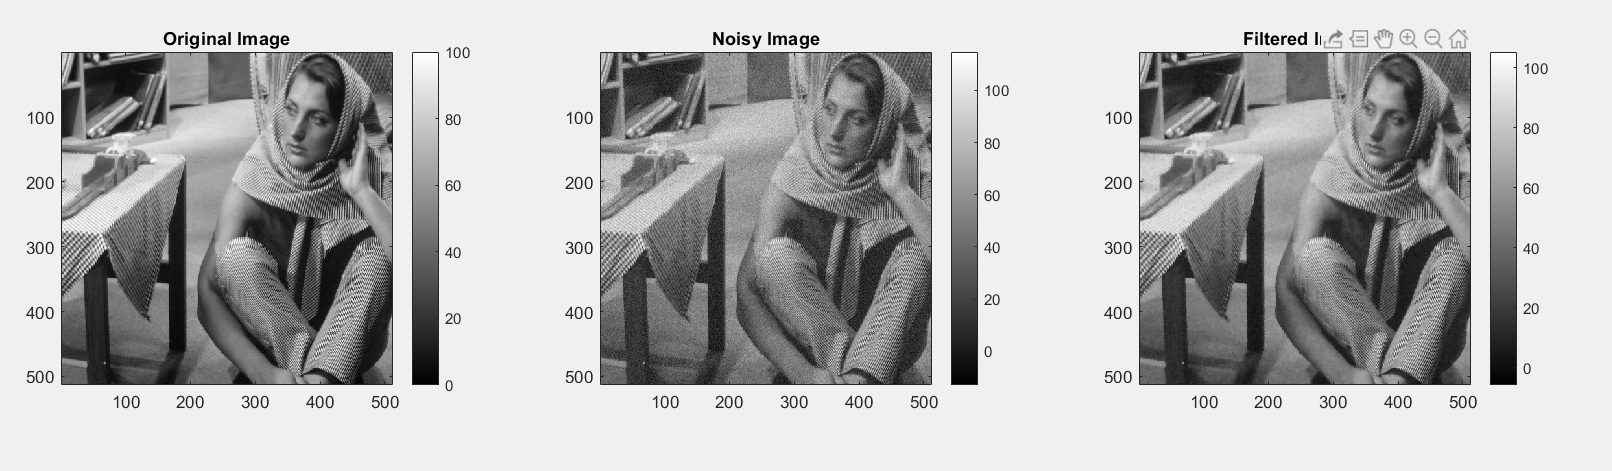
\includegraphics[scale=0.4]{Barbara.png}
    \caption{Barbara Images}
  \label{fig:1}
\end{figure}

\begin{figure}[h!]
  \centering
    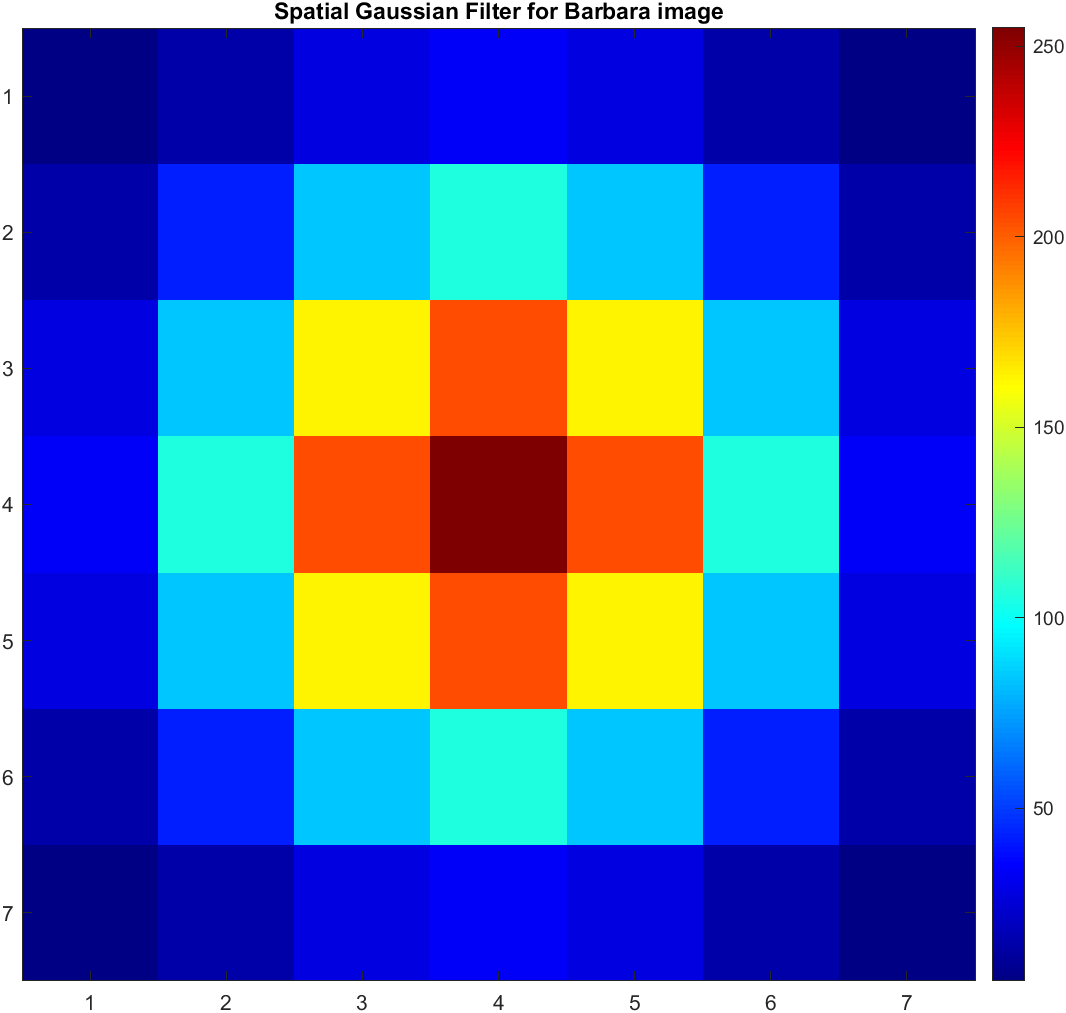
\includegraphics[scale=0.4]{filter_barbara.png}
    \caption{Spatial Gaussian Filter}
  \label{fig:1}
\end{figure}

\subsection*{Grass Image}
We use a window of size 3*3. Standard deviation for spatial filter($\sigma_s)$ is 0.95 while Standard deviation for intensity filter($\sigma_i)$ is 42. RMSD obtained was 7.5410.
\begin{equation*}
    RMSD(0.9*\sigma_s, \sigma_i) = 7.5593\\
\end{equation*}
\begin{equation*}
    RMSD(1.1*\sigma_s, \sigma_i) = 7.5499\\
\end{equation*}
\begin{equation*}
    RMSD(\sigma_s, 0.9*\sigma_i) = 7.5641\\
\end{equation*}
\begin{equation*}
    RMSD(\sigma_s, 1.1*\sigma_i) = 7.5573\\
\end{equation*}

We observe that the parameters obtained produce the least RMSD. Original, Noisy and Filtered image are shown below along with the spatial Gaussian filter. We used color jet to represent it to get better visualization of the filter.
\begin{figure}[h!]
  \centering
    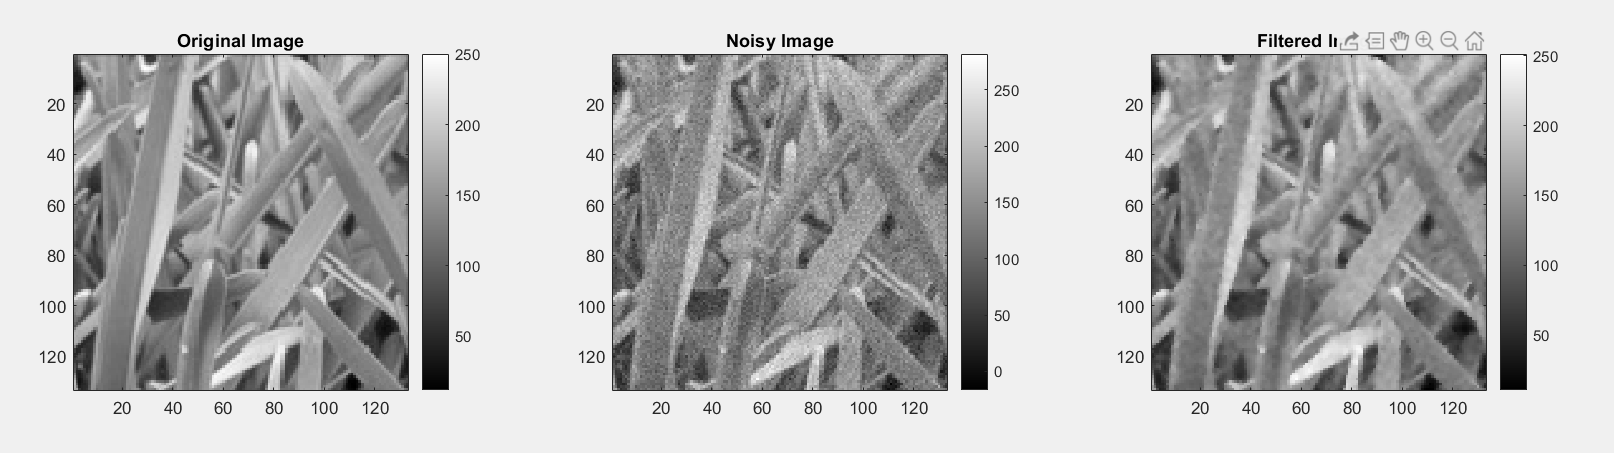
\includegraphics[scale=0.4]{Grass.png}
    \caption{Grass Images}
  \label{fig:1}
\end{figure}

\begin{figure}[h!]
  \centering
    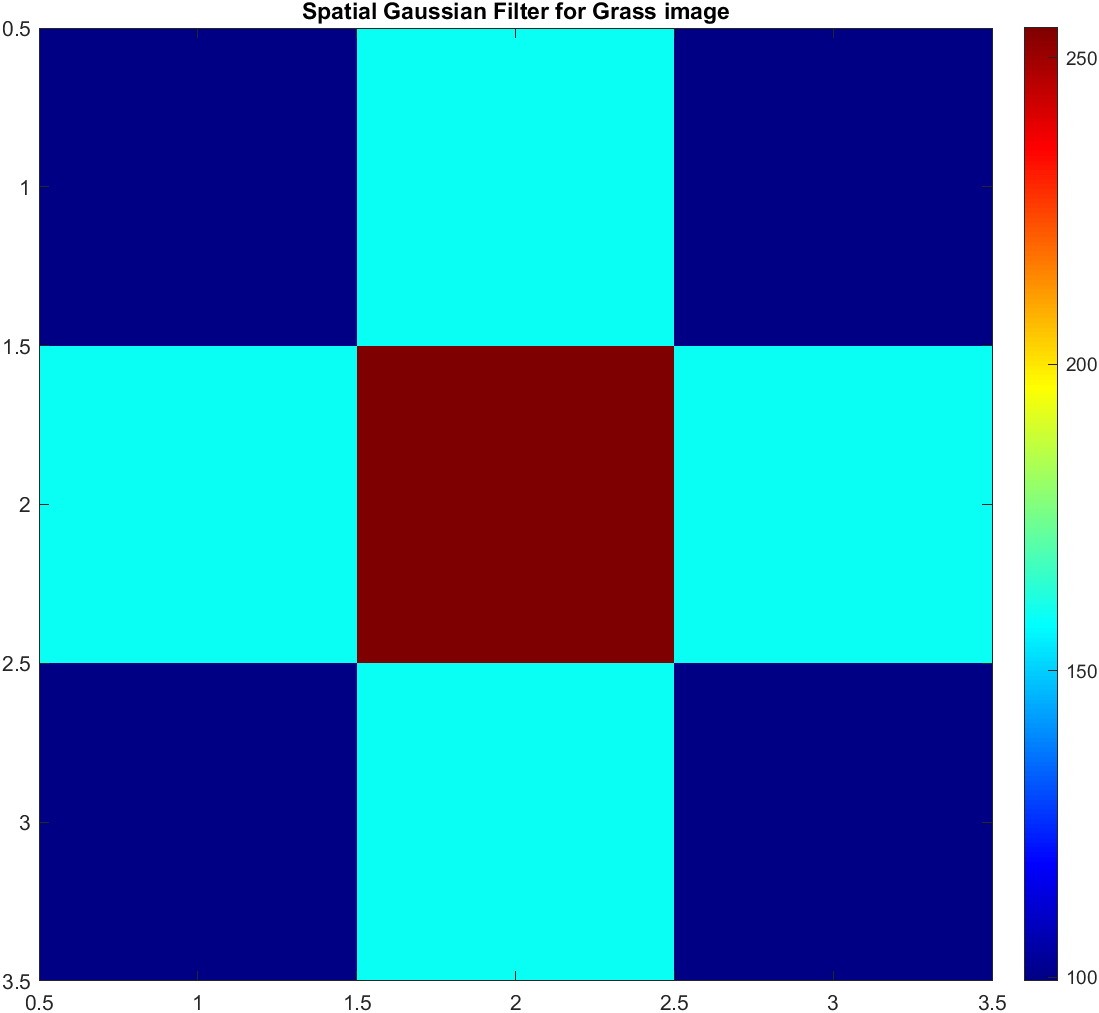
\includegraphics[scale=0.8]{filter_grass.png}
    \caption{Spatial Gaussian Filter}
  \label{fig:2}
\end{figure}

\clearpage

\subsection*{Honey Comb Image}
We use a window of size 3*3. Standard deviation for spatial filter($\sigma_s)$ is 1.25 while Standard deviation for intensity filter($\sigma_i)$ is 40. RMSD obtained was 7.3021.
\begin{equation*}
    RMSD(0.9*\sigma_s, \sigma_i) = 7.3077\\
\end{equation*}
\begin{equation*}
    RMSD(1.1*\sigma_s, \sigma_i) = 7.3047\\
\end{equation*}
\begin{equation*}
    RMSD(\sigma_s, 0.9*\sigma_i) = 7.3246\\
\end{equation*}
\begin{equation*}
    RMSD(\sigma_s, 1.1*\sigma_i) = 7.3299\\
\end{equation*}

We observe that the parameters obtained produce the least RMSD. Original, Noisy and Filtered image are shown below along with the spatial Gaussian filter. We used color jet to represent it to get better visualization of the filter.
\begin{figure}[h!]
  \centering
    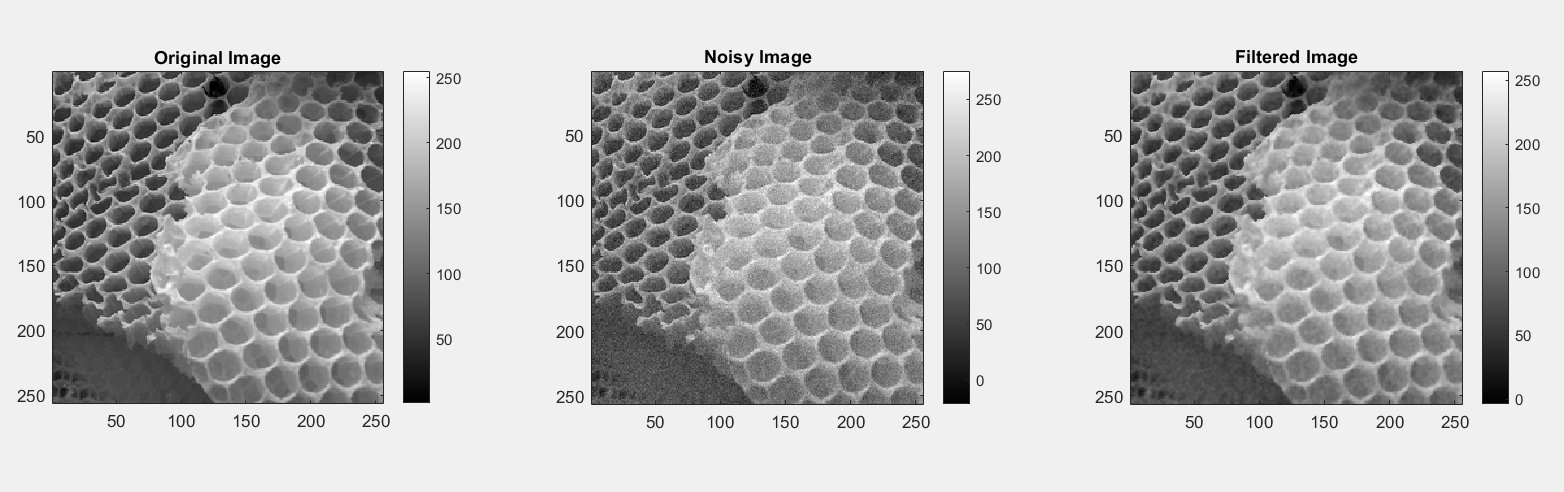
\includegraphics[scale=0.4]{HoneyComb.png}
    \caption{HoneyComb Images}
  \label{fig:1}
\end{figure}
\begin{figure}[h!]
  \centering
    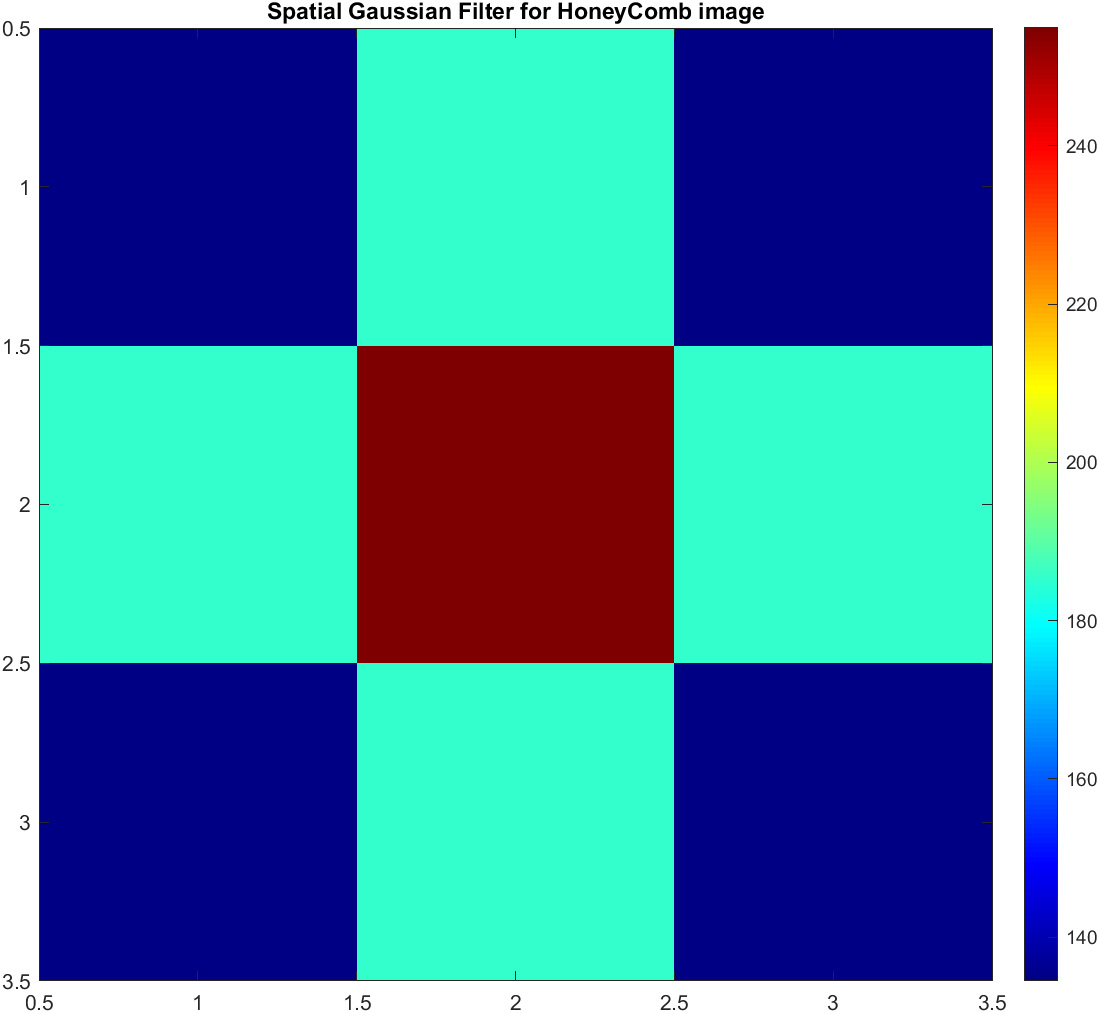
\includegraphics[scale=0.4]{filter_honeyComb.png}
    \caption{Spatial Gaussian Filter}
  \label{fig:3}
\end{figure}

\subsection*{Code Usage}
The main file myMainScript.m is divided into 4 parts. 
\begin{itemize}
    \item Part A (Barbara Image)- This part processes the filtered image for the noisy Barbara Image. We have used a seed to have a constant RMSD every time we run the code. To generate the filtered image the code uses the function myBilateralFiltering which takes  the pixel p, window around that pixel, $\sigma_s$(spatial standard deviation) and $\sigma_i$(intensity standard deviation). It returns the filtered intensity at that point.
    \item Part B (Grass Image)- This part processes the filtered image for the noisy Grass Image. We have used a seed to have a constant RMSD every time we run the code. To generate the filtered image the code uses the function myBilateralFiltering which takes  the pixel p, window around that pixel, $\sigma_s$(spatial standard deviation) and $\sigma_i$(intensity standard deviation). It returns the filtered intensity at that point.
    \item Part C (Honey Comb Image)- This part processes the filtered image for the noisy Honey Comb Image. We have used a seed to have a constant RMSD every time we run the code. To generate the filtered image the code uses the function myBilateralFiltering which takes  the pixel p, window around that pixel, $\sigma_s$(spatial standard deviation) and $\sigma_i$(intensity standard deviation). It returns the filtered intensity at that point.
    \item Part D (Spatial Filters)- This part generates the spatial Gaussian filters as an image for visualization. We use colorjet to have better visualization.
\end{itemize}

\end{document}
